\documentclass[]{final_report}
\usepackage{graphicx}
\usepackage{hyperref}
\usepackage{listings}
\usepackage{graphicx}
\usepackage[backend=bibtex]{biblatex}
\addbibresource{refs.bib}


%%%%%%%%%%%%%%%%%%%%%%
%%% Input project details
\def\studentname{James Arnott}
\def\reportyear{2022}
\def\projecttitle{Comparison of Image Classification Models with Transfer Learning}
\def\supervisorname{Li Zhang}
\def\degree{BSc (Hons) in Computer Science}
\def\fullOrHalfUnit{Full Unit} % indicate if you are doing the project as a Full Unit or Half Unit
\def\finalOrInterim{Interim Report} % indicate if this document is your Final Report or Interim Report

\begin{document}

\maketitle

%%%%%%%%%%%%%%%%%%%%%%
%%% Declaration

\chapter*{Declaration}

This report has been prepared on the basis of my own work. Where other published and unpublished source materials have been used, these have been acknowledged.

\vskip3em

Word Count:

\vskip3em

Student Name: \studentname

\vskip3em

Date of Submission:

\vskip3em

Signature:
\begin{figure}[ht!]
  
\includegraphics[width=50mm]{images/signature.jpg}
\end{figure}

\newpage

%%%%%%%%%%%%%%%%%%%%%%
%%% Table of Contents
\tableofcontents\pdfbookmark[0]{Table of Contents}{toc}\newpage

%%%%%%%%%%%%%%%%%%%%%%
%%% Your Abstract here

\begin{abstract}

  Transfer learning is a common, efficient method for training deep learning models.
  It involves using a pre-trained model to extract features from a dataset,
  and then training a new model on top of the extracted features.
  This report compares a variety of different image classification models with transfer learning,
  and evaluates their performance on a dataset of images of flower species and MRI scans of Alzheimer's patients brains.

\end{abstract}
\newpage

%%%%%%%%%%%%%%%%%%%%%%
%%% Project Spec

\chapter*{Project Specification}
\addcontentsline{toc}{chapter}{Project Specification}
Your project specification goes here.

%%%%%%%%%%%%%%%%%%%%%%
%%% Introduction
\chapter{Introduction}

\section{What transfer learning is}
Transfer learning is a common, efficient method for training deep learning models.
There are many different ways to implement transfer learning and here I hope to compare the performance
of a variety of different methods with different pre-trained models.

The applications for transfer learning are vast, and it is a common method for training deep learning models,
This is because it is a very efficient method for training models as most of the work is done by the pre-trained model.
The pre-trained model is used to extract features from the dataset, and then a new model is trained on top of the extracted features.
The pre-trained model is usually frozen so that it does not change during training, and only the new model is trained.

After the new model is trained on top, a process known as fine-tuning can be used to further improve the performance of the model.
Fine-tuning involves training the new model on the dataset, but with a lower learning rate than the initial training.
This is also where the model is usually unfrozen, so that the pre-trained model can be trained as well, which helps to improve the overall performance of the model.

\section{The Models I will be comparing}
The models I have chosen to compare are the MobileNetv3Small\cite{DBLP:journals/corr/abs-1905-02244}, MobileNetv3Large\cite{DBLP:journals/corr/abs-1905-02244}, ResNet50\cite{DBLP:journals/corr/HeZRS15}, ResNet10\cite{DBLP:journals/corr/HeZRS15}, ResNet152\cite{DBLP:journals/corr/HeZRS15}, and InceptionV3\cite{DBLP:journals/corr/SzegedyVISW15} models.
These models are all pre-trained on the ImageNet dataset, which contains 1.2 million images of 1000 different classes.

\section{The Datasets I will be using}
The datasets I have chosen to use for this project are the Oxford 102 Flower Dataset\cite{OxfordFlowers102} and the Alzheimer's MRI Dataset\cite{AlzheimersDataset}.

The choice of datasets is based on the fact that they are both image classification datasets they are both relatively small in classes and
the they have a variety classes ranging in difficulty, which will allow me to compare the capabilities of the different models in a variety of different scenarios.

\chapter{The way Neural Networks work}
\begin{figure}[ht!]
  \centering
  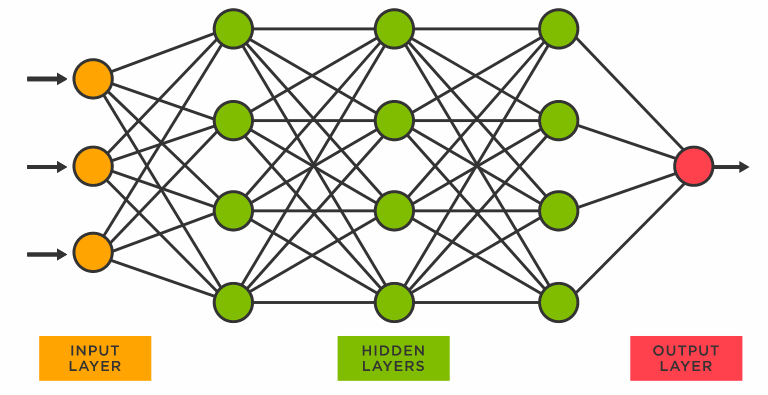
\includegraphics[width=100mm]{images/NeuralNetwork.png}
  \caption{A diagram of a neural network \cite{NeuralNetworkDiagram}}
\end{figure}

\section{What is a Neural Network}
A neural network is a machine learning model that is inspired by the way the human brain works.
It is made up of a series of layers, each layer is made up of a number of neurons.
Each neuron is connected to every neuron in the next layer, and each connection has a weight associated with it.
The weights are used to determine how much each neuron in the next layer is affected by the current neuron.
The weights are updated during training, and the process of updating the weights is known as backpropagation.

\section{What is a Convolutional Neural Network}
A convolutional neural network (CNN) is a type of neural network that is used for image classification.
It is made up of a series of convolutional layers, pooling layers, and fully connected layers.
The convolutional layers are used to extract features from the image, and the pooling layers are used to reduce the size of the image.
The fully connected layers are used to classify the image.
They are often much more efficient than other types of neural networks, and are commonly used for image classification.

\chapter{Transfer Learning}

\section{Why use Transfer Learning}
Transfer learning can enable a model to be trained much more efficiently than if it was trained from scratch, as most of the work is done by the pre-trained model.
Aside from the extra time it takes to train a model from scratch, it often requires more training data, which is not always available and can be expensive to obtain.
Transfer learning can often get better results than training a model from scratch, as the pre-trained model has already learned about different features from a large dataset,
and the transfer learning model can then use these features to learn about the new dataset.

\section{Drawbacks of Transfer Learning}
The main drawback of transfer learning is that it is not always possible to use it,
as the pre-trained model may not be able to extract the features from the new dataset.
With image classification, the pre-trained model can typically extract features from any image, but it may not be able to extract the features that are needed for the new dataset.
Transfer learning can also be less efficient than training a model from scratch, 
as the pre-trained model will have all the weights from the original dataset, which may not be needed for the new dataset.
This can cause the model to be less efficient, as it will have to train on weights that are not 
needed but will still affect the performance of the model.

\pagebreak
\section{The code behind the transfer learning}
The code for the transfer learning is shown below.

\begin{lstlisting}[language=Python]
  # This imports the model from the keras library
  MobileNetV3Small = keras.applications.MobileNetV3Small(
    input_shape=(224, 224, 3),
    include_top=False, 
    weights='imagenet')

  # Create the model
  model = keras.Sequential()

  # Freezing all but 10 layers of the pre-trained model
  for layer in MobileNetV3Small.layers[:-10]:
    layer.trainable = False

  # Adding the pre-trained model to the model, along with 
  # a dropout layer and a fully connected layer
  model.add(MobileNetV3Small)
  model.add(keras.layers.Flatten())
  model.add(keras.layers.Dense(512, activation='relu'))
  model.add(keras.layers.Dropout(0.6))
  model.add(keras.layers.Dense(512, activation='relu'))
  model.add(keras.layers.Dropout(0.6))
  model.add(keras.layers.Dense(4, activation='softmax'))
\end{lstlisting}

The code above shows how to create a model using transfer learning,
creating the model structure consists of adding the pre-trained model to the model, 
and then adding a few layers on top of it. The flatten layer is used to flatten the output of the pre-trained model
as that is the input for the fully connected layers. The fully connected layers are used to classify the images.

The dropout layers are used to prevent overfitting, and the dense layers are used to classify the images.
The dense layers are potentially the most important part of the model, as they are the ones that are actually learning about the dataset.
They get trained on the features extracted by the pre-trained model, and the weights of the dense layers are what is used to classify the images.

The final layer of the model is a softmax layer, which is used to classify the images.
It is used to classify the images into one of the classes in the dataset, in this example,
the 4 levels of Alzheimer's disease that are in the Alzheimer's MRI Dataset.

\pagebreak
\section{How to implement Transfer Learning}

\subsection{Extracting features}
Feature extraction is the process of using a pre-trained model to extract features from a dataset.
The pre-trained model is usually frozen so that it does not change during training, and only the new model is trained,
and the new model is trained on top of the extracted features.

\subsection{Fine-tuning}
This is the process of training the new model on the dataset, but with a lower learning rate than the initial training and the model is usually unfrozen,
so that the pre-trained model can be trained as well, which helps to improve the overall performance of the model.
This was where I managed to get the best results for my models.

\section{How to fine-tune a model}
Fine-tuning a model is a very simple process, and can be done in just a few lines of code.
The first step is to unfreeze the pre-trained model, which can be done by setting the trainable attribute of the layers to True.
The next step is to set the learning rate to a lower value, which can be done by setting the learning rate attribute of the optimizer.
The final step is to recompile the model, which can be done by calling the compile method of the model.
Here is an example of how I fine-tuned a model using keras:

\begin{lstlisting}[language=Python]
  base_model.trainable = True
  optimizer.learning_rate = 0.0001
  model.compile(optimizer=optimizer, loss=loss, metrics=metrics)
\end{lstlisting}

\begin{verbatim}
  base_model.trainable = True
  optimizer.learning_rate = 0.0001
  model.compile(optimizer=optimizer, loss=loss, metrics=metrics)
\end{verbatim}

\section{The different structures of the models}
There are so many different ways to structure a model and they can 

\chapter{Evaluating the performance}

\section{The different metrics}
% Accuracy
Accuracy is the most common metric used to evaluate the performance of a model, and is defined as the number of correct predictions divided by the total number of predictions.
It is a very simple metric to understand, and is therefore often used to compare the performance of different models.
There is accuracy for both the training and validation sets, and the accuracy of the validation set is used to determine how well the model generalises to new data,
and a validation accuracy that is much lower than the training accuracy is a sign that the model is overfitting.
However, it is not always the best metric to use, as it can be misleading in some cases.

% Loss
Loss is the most common metric used to evaluate the performance of a model, it is calculated by taking the difference between the predicted value and the actual value.
There are however many different types of loss functions, and the one that is used depends on the type of problem that is being solved.
These could be binary cross entropy, categorical cross entropy, or mean squared error. For my project I used binary cross entropy due
to it's simplicity and the fact that it is the most common loss function used for binary classification problems.

% Validation vs Training Loss and Accuracy
The validation loss and accuracy are used to determine how well the model generalises to new data, and a validation loss that is much higher than the training loss is a sign that the model is overfitting.
For the validation set, I have assigned 20\% of the data to be used.

% Confusion Matrix
The confusion matrix is a table that shows the number of correct and incorrect predictions for each class.
It is a very useful metric to use when evaluating the performance of a model, as it can show which classes the model is having the most trouble with.

\section{Data Augmentation}

Data augmentation is the process of artificially increasing the size of a dataset by applying random transformations or filters to the images.
This can help to improve the performance of a model, as it can help to reduce overfitting, and can also help to improve the generalisation of the model.
The transformations that are applied to the images are usually random, and can include things like rotating the image, 
flipping the image, or changing the contrast/saturation of the image.

In the case of the Alzheimer's MRI Dataset, it is extremley useful to have more data to train the model on, as there are a limited number of brain scans available.
MRI scans are also very expensive, so using data augmentation can significantly reduce the cost of training the model.

In the Alzheimer's MRI Dataset, the majority of the archive is comprised of augmented images already so I did not need to apply any data augmentation to the images.

\section{Evaluating the given metrics}
The metrics of accuracy and loss generally tell us how well the model is performing,
but they do not tell us how well the model is performing for each class.
They do also not tell us how well the model would work in a real world scenario, 
as they are only calculated on the training and validation sets, of which we have a limited amount of data.

The validation dataset is also from the same distribution as the training dataset, 
so it is not a good representation of how well the model would work in a real world scenario 
as the scans could be of a different quality.

I have used the augmented dataset for the training and validation sets as this 
should give a better representation of how well the model would work in a real world scenario.

\begin{figure}[ht!]
  \centering
  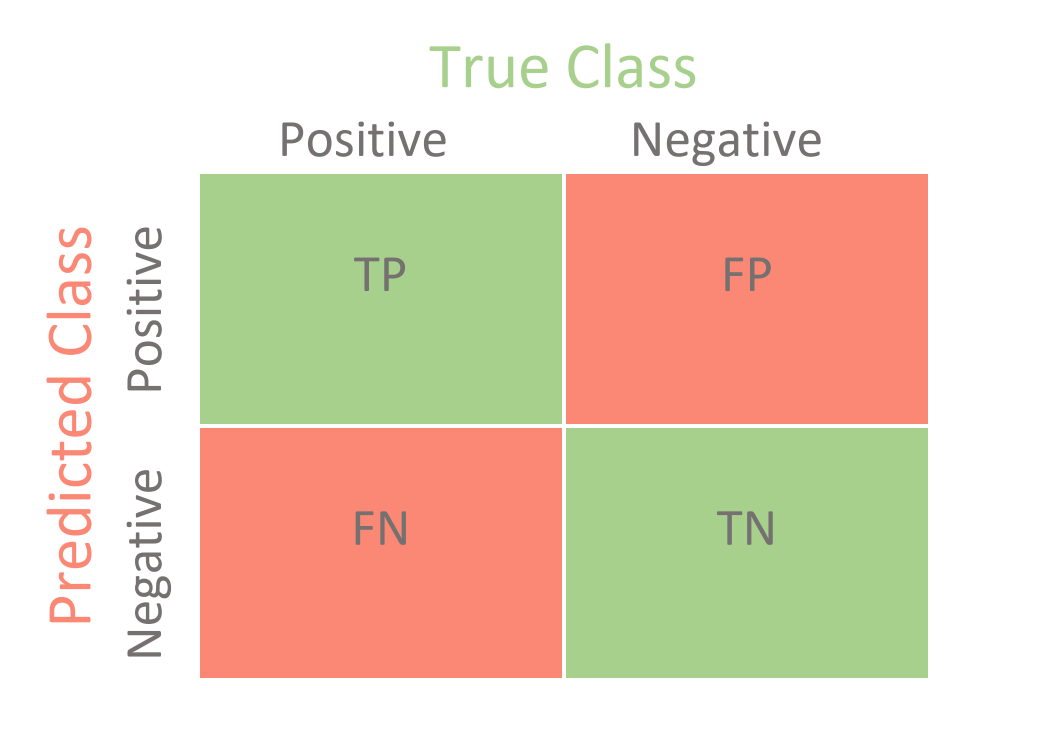
\includegraphics[width=100mm]{images/ConfusionMatrix.png}
  \caption{A confusion Matrix\cite{ConfusionMatrix}}
\end{figure}

\section{The different datasets}

\section{The different sizes and structures of the models}

\section{The different optimizers}

\chapter{Optimising the models}
% talk about the different optimizers and how they affect the performance of the models
% Also talk about the different learning rates and how they affect the performance of the models

\chapter{Conclusion}

This project is a great learning experience for me, and I have learned a lot about transfer learning and how to implement it.
Before I started this project, I had never used transfer learning before, and had only used pre-trained machine learning models for image classification.
I have learned a lot about the different types of models, how they are structured, and how they can be used for transfer learning.

\section{What I have learned}
I have specifically learnt how complex image classification models are structured, as they are far more complex than I had initially thought.
% talk about mobilenetv3

\section{What I will do differently}
I need to spend more time researching the different structures of the models, and how the optimal ways they can be used for transfer learning.


\section{What I need to do next}



\newpage
\printbibliography
\label{endpage}
\end{document}
\end{article}